\subsubsection{\stid{4.14} ECP SZ: Fast, Effective, Parallel Error-bounded Exascale Lossy Compression for Scientific Data}

\paragraph{Overview}

Extreme scale simulations and experiments are generating more data than can be stored, communicated and analyzed. Error-bounded lossy compressor is critical because it can get a very high compression ratio while still respecting data fidelity based on user's requirement on compression errors. 
%Current lossless compression methods suffer from low compression ratio and do not adequately address the limitations in storage bandwidth and storage space of projected exascale systems. Existing lossy compressors are not covering the needs of many ECP applications.

The VeloC-SZ project is extending and improving the SZ error-bounded lossy compressor for structured and unstructured scientific datasets. SZ offers an excellent compression ratio as well as very low distortion and compression time. Further work is essential, however, to improve our SZ lossy compressor for ECP scientific datasets, while ensuring that user-set error controls are respected. Specifically, we are: (i) optimizing SZ compression ratios, accuracy and speed based on end-user needs (ii) refactoring SZ in C++ to support a composable compression framework and all data types used in ECP applications, (iii) integrating SZ in ECP client applications, (iv) developing the GPU version of SZ which supports multiple supercomputers with different architectures (such as Aurora, Frontier and Summit), and (v) improving robustness and testability. %Our goal is to produce a high-quality lossy compressor responding to the needs of ECP exascale applications and experiment users. To this end, 
We are working with multiple ECP application teams, including ExaSky cosmology teams (HACC), molecular dynamics simulations groups (EXAALT), x-ray laser imaging experimentalists (ExaFEL), and computational chemists (NWChem-X, GAMESS) to optimize SZ for their applications and to harden SZ.

\paragraph{Key Challenges}

SZ faces several key challenges:
\begin{itemize}
\item \textbf{Improving Prediction Accuracy} The core step in SZ is the point-wise data prediction for different datasets. The higher the prediction accuracy, the higher the compression quality in general. However, how to design an effective predictor that can adapt to diverse datasets is very challenging.
\item \textbf{Parameter tuning}: One challenge in optimizing lossy compression for scientific applications is the large
diversity of scientific data, dimensions, scales, and dynamic data changes in both space and time. Each application requires specific parameters tuning and in some cases, a specific compression pipeline, which is non-trivial to implement.
\item \textbf{Implementation \& optimization over GPU}: The third challenge is the sophisticated design in different stages of the SZ (such as data prediction, Huffman tree construction, Huffman encoding), which makes the development of efficient GPU kernels non-trivial. 
\item \textbf{Diverse integration schemes}: The fourth challenge is the diversity of the integration schemes for the different ECP client applications: HACC integrates SZ in a proprietary I/O library (GIO), Exafel integrates SZ directly in the LCLS data processing pipeline. GAMESS integrates SZ in the application directly replacing some code sections. EXAALT integrates SZ for saving storage space.
\item \textbf{Portable support for GPU}: Optimization of SZ for Aurora and Frontier requires writing portable accelerator codes that are non trivial for complex compression pipeline. 
\item \textbf{Improve development robustness and testability}: The SZ testing infrastructure (unit test, correctness test, performance test, regression test, continuous integration) will need to be adapted and its performance optimized for the new C++ implementation. A template based approach must be used to improve robustness, debugging and testability.
\end{itemize}

\paragraph{Solution Strategy}

As for the first two challenges, we develop a novel, adaptive predictor based on a dynamic spline interpolation which is combined with the classic Lorenzo predictor, such that the rate distortion (bit rate vs. data distortion PSNR) can be improved significantly.

As for the third challenge, we keep exploring the new strategies to improve the GPU kernel performance especially for bottleneck stages of cuSZ -- GPU version of SZ. This requires in-depth understanding of the bottleneck of cuSZ and numerous performance tuning tests to explore new strategies.   

As for the fourth challenge, we refactor SZ in C++, starting from the current C version. This refactoring is the perfect occasion to implement a new more modular design of SZ, capable of integrating more stages in the compression pipeline and of selecting compression stages based on specific application data features.

Concerning the fifth challenge, we are in contact with ALCF and OLCF as well as with vendors to access simulators and early systems. We also develop the portable GPU implementation of SZ for different GPUs by leveraging corresponding libraries/toolkits such as oneAPI and HIP.

We are continuously improving the robustness and testability. We integrated SZ into ORNL CI environment, and often discuss potential issues with application teams when needed. 

\paragraph{Recent Progress}

We summarize all 10+ different versions of SZ in our official website (http://szcompressor.org), including CPU version, GPU version, customize version for applications such as EXAALT and GAMESS. 
%Specifically, The flagship products include CPU version of SZ (the classic C version), composable version of SZ (a.k.a., SZ3 in C++), dynamic interpolation based SZ -- Interp-SZ (particularly effective for Seismic imaging data and turbulent flow data), CUDA version of SZ -- cuSZ, Kokkos version of SZ, ultrafast version of SZ -- SZx, specific version customized for GAMESS -- Pastri-SZ, specific version customized for ExaFEL -- Roibin-SZ, specific version customized for ExaLT -- MMD-SZ, FPGA version of SZ -- waveSZ, etc. 

We significantly improved compression quality and performance for SZ. (1) We improved the rate distortion significantly by a dynamic spline interpolation method, which is particularly effective in compressing smooth datasets with wave patterns such as turbulent flow data and quantum chemistry data (QMCPack). (2) We customized an effiicent error-bounded lossy compressor - called MMD-SZ for molecular dynamics (MD) applications such as LAMMPS and ExaALT, by leveraging the potential data characteristics of MD simulation datasets. The compression ratio has been improved by about 100+\% over the generic version of SZ. 

We have developed SZ3, which breaks down different stages of SZ to form a loosely-coupled model, such that the users can construct a new compressor by customizing each compression step conveniently. %By leveraging the SZ3 to compose new compression pipeline, we have successfully developed MMD-SZ for MD simulation datasets, which can improve the compressio ratio by 100+\% with the same distortion, and also improved the compression quality significantly for Advanced photon Source (APS) datasets.

We also significantly improved the GPU kernel performance of SZ's compression stage. We have released the cuda-based SZ (cuSZ) 0.2.9.1 and tested its performance on V100 GPU and A100 GPU. We identified that the bottleneck of cuSZ is its Huffman encoding stage and dictionary encoding stage. (1) We develop an efficient parallel codebook construction on GPUs that scales effectively with the number of input symbols. (2) We propose a novel reduction based encoding scheme that can efficiently merge the codewords on GPUs. (3) We optimize the overall GPU performance by leveraging the state-of-the-art CUDA APIs such as Cooperative Groups. (4) We evaluate our Huffman encoder thoroughly using six real-world application datasets on two advanced GPUs and compare with our implemented multi-threaded Huffman encoder. Experiments show that our solution can improve the encoding throughput by up to 5.0$\times$ and 6.8$\times$ on NVIDIA RTX 5000 and V100, respectively. Figure \ref{fig:sz-huffman} illustrates the parallel design of the Huffman encoding in cuSZ. 
\begin{wrapfigure}{l}{0.47\textwidth}
  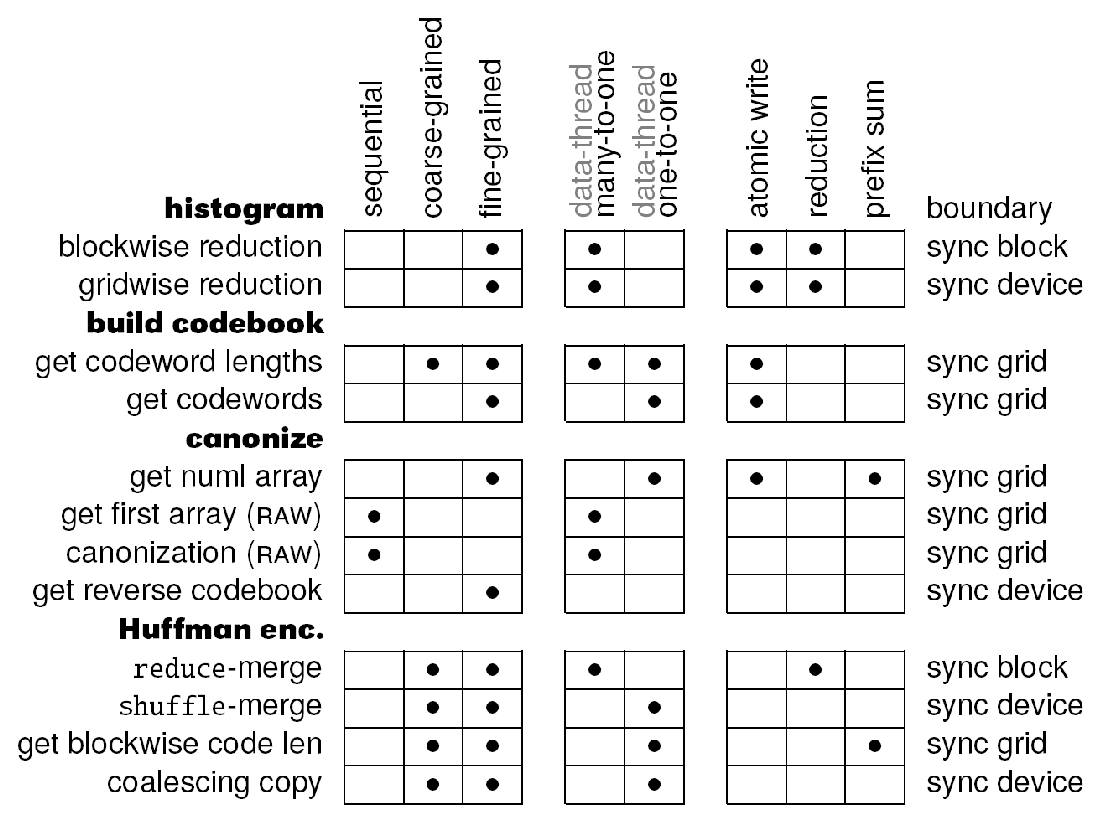
\includegraphics[width=0.4\textwidth]{projects/2.3.4-DataViz/2.3.4.14-VeloC-SZ/SZ-Huffman}
  \caption{Parallelism implemented for Huffman coding’s subprocedures (kernels).
``sequential” denotes that only 1 thread is used due to data dependency.
``coarse-grained” denotes that data is explicitly chunked. ``fine-grained” denotes
that there is a data-thread mapping with little or no warp divergence.}%
  \label{fig:sz-huffman}%
\end{wrapfigure}


We also signficantly improved the GPU kernel performance for SZ's overall workflow and decompression stage in particular. (1) We propose an efficient compression workflow to adaptively perform run-length encoding and/or variable-length encoding. (2) We derive Lorenzo reconstruction in decompression as multidimensional partial-sum computation and propose a fine-grained Lorenzo reconstruction algorithm for GPU architectures. (3) We carefully optimize each kernel by leveraging state-of-the-art CUDA parallel primitives. (4) We evaluate the new version of cuSZ using seven real-world HPC application datasets on V100 and A100 GPUs. Experiments show the new implementation improves the compression throughputs and ratios by up to 18.4$\times$ and 5.3$\times$, respectively on the tested datasets.

Experiments on A100 GPU show that cuSZ's overall performance reaches up to 84$\sim$92GB/s based on both HACC and NYX datasets.

We ported cuSZ in active development onto the new backend: native DPC++, for the A21 platform. 
DPC++ along with oneAPI SDK serves as the native programming language on A21 system. From DPC++ setup, we successfully executed our prototype kernels that can partially match the native CUDA kernel executed on NVIDIA V100.

We developed CI for SZ on ORNL CI environment and also added smoke test to Spack for SZ. 

\paragraph{Preliminary Experiences on Early Access systems}
We translated the CUDA-version of SZx (cuSZx) to the HIP-version SZx (hipSZx), then successfully compiled it. To accomplish the translation, we leveraged HIPIFY. There are two tools in HIPIFY: hipify-perl and hipify-clang. We first tried hipify-perl on the Crusher cluster. It is a regular expression-based translator and does not rely on the CUDA toolkits (there is no CUDA module on Crusher). Unfortunately, the hipify-perl translated code yielded many errors during the compilation since this translator only performed simple string replacement without any syntax checks. Hence, we had to use hipify-clang to translate the code again on Summit (it requires a CUDA toolkit). The converted code can be compiled with hipcc on Crusher after moderate adjustments. During the compilation, we observed that the default rocm/4.2.0 does not work with our code; we have to load the module rocm/4.5.0 or above versions. With the new rocm version, we had to specify the running platform. For example, we need to define \_\_HIP\_PLATFORM\_AMD\_\_ before the main function in hipSZx in order to run it on Crusher. We note that the translated files should be saved in .cpp format. The default .hip and the .c suffixes do not work as the compiler cannot recognize the GPU-related code snippets in these file formats. There were some known unsupported CUDA instructions in HIP, for instance, the cooperative groups and the warp-level shuffle operations. We had to avoid them for now.

The generated executable files were runnable. However, there were memory access faults that happened during the execution and made the program crash. We had spent some time debugging it and figured out that it was caused by the indexing issue when reading an array in the GPU kernel. These indices were calculated by a GPU-based prefix scan step which frequently used the warp-level shuffle operations. The CUDA shuffles enabled explicit warp synchronization and used masks to allow partial warp shuffling. On the contrary, HIP only implemented the old fashion shuffles that had been deprecated in CUDA. These HIP shuffles did not allow masks and thus needed to involve the entire warp every time. Therefore, the straightforward translation from the CUDA shuffles to the HIP shuffles made the results incorrect in our GPU prefix scan. We have to find a way to work around it, e.g., move the prefix scan data from the registers to the shared memory. But this will obviously downgrade the overall performance.


\paragraph{Next Steps} Our next efforts include: (1) Improve compression quality and performance for cuSZ, (2) Keep working on the compression quality improvement and integration of SZ in more ECP applications such as ExaFEL and EXAALT, and (3) evaluate the portable GPU version of SZ on ECP platforms.

